\section{``Sample" vs ``Population''  distribution of the signal}\label{sec:sampledistribution}

The observation consists of the realisations of the random variables $\Sample$ and $\Signal[\Sample]$. In this section, we derive the distribution of the observed values of the signal on the sample, (e.g. the distribution of $\Signal[\Sample]$) from  the distribution of the design variable conditionally $\Desvar$ to the signal $\Signal$ and the function that links the design to the design variable, or equivalently the distribution of the sample $\Sample$ conditionally to the design variable $\Desvar$. We resort to  the Bayes formula to express the density of $(\Signal[\Sample],\Sample)$ in $(\signal,\position)$,   as the product of the density of the sample $\Sample$ in $\position$ conditionally on $\Signal[\position]=\signal$ by the density of the signal $\Signal[\position]$ in $\signal$. 
\subsection{Density ratio}
\subsubsection{Definition and properties}
%In this section, we derive the distribution of the observed values of the signal on the sample, (e.g. the distribution of $\Signal[\Sample]$) from  the distribution of the design variable conditionally $\Desvar$ to the signal $\Signal$ and the function that links the design to the design variable, or equivalently the distribution of the sample $\Sample$ conditionally to the design variable $\Desvar$. To this end, we proceed step by step and resort to the Bayes formula. 
We start with the following definition.


%{\color{red} Do we need the notation g ? the idea is that $g$ is the density for the sample. I am in favour of creating a command and call it $\pi$ instead.} 


\begin{definition}
For a random set $\Sampleindex$, 
define
$\densityratio_{\Sampleindex}(.\mid.)$ as any function that satisfies:

\begin{equation}
P^{(\Sample_\Sampleindex,\Signal[\Sample_\Sampleindex])}-\text{a.s}(\position,\signal),~\density_{\Signal[\position]\mid\Sample_\Sampleindex=\position}\left(\signal\right)=
    \density_{\Signal[\position]}\left(\signal\right)
    \densityratio_{\Sampleindex}\left(\position\mid  \signal\right)\label{eq:owijoj}
\end{equation}

\end{definition}


\begin{property}\label{prop:ieuhierhgi}
%Let $\Sampleindex$ be a non random finite subset of $\mathbb{N}$, then
\begin{equation}
P^{(\Sample_\Sampleindex,\Signal[\Sample_\Sampleindex])}-\text{a.s}(\position,\signal),~~~
\densityratio_{\Sampleindex}\left(\position \mid \signal\right)
         \density_{\Sample_\Sampleindex}\left(\position\right)=
    \density_{\Sample_\Sampleindex\mid \Signal[\position]}\left(\position|\signal\right)
\end{equation}


\end{property}

\begin{proof}
From the Bayes formula:
\begin{eqnarray}
\density_{\Signal[\position]\mid\Sample_\Sampleindex =\position }\left(\signal\right)
&=&(\density_{\Sample_\Sampleindex }(\position))^{-1}~\density_{\Signal[\position],\Sample_\Sampleindex }(\signal,\position)\\
&=&(\density_{\Sample_\Sampleindex }(\position))^{-1}~
\density_{\Sample_\Sampleindex \mid\Signal[\position]}(\position\mid \signal)~
\density_{\Signal[\position]}(\signal)\label{eq:oijoijsf}
\end{eqnarray}


So, combining Equations \eqref{eq:oijoijsf} and  \eqref{eq:owijoj}:
\begin{equation}
{\densityratio_{\Sampleindex}\left(\position \mid \signal\right)}
=(\density_{\Sample_\Sampleindex }(\position))^{-1}
~\density_{\Sample_\Sampleindex \mid\Signal[\position]}(\position\mid \signal).
\end{equation}
\end{proof}%

Property \ref{prop:ieuhierhgi} provides an interpretation of $\densityratio_\Sampleindex(\signal\mid \position)$ as the probability that the draws indexed by $\Sampleindex$ correspond to the sample $\position$ conditionally on the values of $\Signal$ in $\position$ divided by the same probability unconditionally on the values of $\Signal$. 
In this sense, the density ratio $\densityratio_\Sampleindex(\signal\mid \position)$ is a relative probability of selection.
%$\densityratio_{\Sampleindex}(\position\mid\signal)$




%Besides,
%\begin{equation}\label{eq:iurhiehgieurhg}
%\density_{\Sample_\Sampleindex }(\position)=
%\int \density_{\Sample_\Sampleindex \mid \Signal[\position]}(\position\mid \signal)~ \density_{\Signal[\position]}(\signal)~
%\derive \dominantY^{\otimes \Sampleindex}(\signal)
%\end{equation}
\begin{property}
The density ratio $\densityratio$ can be derived from the distribution of $\Desvar$ via:

\begin{eqnarray}\label{eq:rho_expression}
\densityratio_{\Sampleindex}(\position\mid\signal)&=&\left({\int
         \density_{\Sample_\Sampleindex\mid \Desvar}\left(\position|\desvar\right)\derive P^{\Desvar}}\right)^{-1}{\int\density_{\Sample_\Sampleindex\mid \Desvar}(\position\mid\desvar)\derive P^{\Desvar\mid\Signal[\position]=\signal}(\desvar)}
\label{eq:oigjeogjio}\end{eqnarray}
\end{property}

\begin{property}\label{prop:indeprho}
If $\Desvar$ and $\Signal$ are independent, then $\densityratio_K(\position\mid\signal)=1$.
\end{property}
\begin{proof}
$\Desvar\perp\Signal\Rightarrow P^\Desvar=P^{\Desvar\mid\Signal[\position]=\signal}$. Replacing $P^{\Desvar\mid\Signal[\position]=\signal}$ by $P^{\Desvar}$ in the numerator of Equation \eqref{eq:rho_expression} yields  $\densityratio_K(\position\mid\signal)=1$.
\end{proof}

\subsubsection{Computation of $\densityratio$ on a Case study}
In this subsection, we use the framework of Example \ref{example:2.4} to illustrate the properties and provide graphical representations of the density ratio.
We remind that in this framework, $\Sample\sim \mathrm{Ppp}(\Desvar)$ or  $\Sample\sim \mathrm{bpp}(\Desvar,\samplesize)$.
Conditionally on $\Signal[\position]=\signal$, $\Desvar$ is a log normal random process with distribution characterized by 
$E[\log(\Desvar[\position'])\mid \Signal[\position]=\signal]=\paramnuisance_0+\paramnuisance_1(\mu+\Sigma_{\position',\position}\Sigma_{\position,\position}^{-1} (\signal-\mu))$ and 
$\mathrm{Var}[\log(\Desvar[\position'])\mid \Signal[\position]=\signal]=\paramnuisance_2^2\provar_{\varepsilon;\position',\position'}+\paramnuisance_1^2\left(\provar_{\Signal;\position',\position'}-\provar_{\Signal;\position',\position}\provar_{\Signal;\position,\position}^{-1}\provar_{\Signal;\position,\position'})\right)$.
\begin{proof}
See Appendix \ref{sec:A.owifjoeij}
\end{proof}

For $\position=\mathbf{0}$  and  $\signal=\mathbf{0}$,
\begin{eqnarray*}
\lefteqn{\density_{\Sample_{\{1\}}\mid\Signal[\mathbf{0}]=\mathbf{0}}(\mathbf{0}))}\\&=&
\density_{\Sample_{\{1\}}}(\mathbf{0})\\
&=&\left|\begin{array}{ll}
\int \exp\left(-(\desvar.\dominantU)(\Pop)\right)\derive P^{\Desvar}(\desvar)&\text{if }\Sample\sim\mathrm{Ppp}(\Desvar)\\
0&\text{if }\Sample\sim\mathrm{bpp}(\Desvar,\samplesize),\end{array}\right.
\end{eqnarray*}
so $\densityratio_{\{1\}}(\mathbf{0}\mid\mathbf{0})=
\density_{\Sample_{\{1\}}\mid\Signal[\mathbf{0}]=\mathbf{0}}(\mathbf{0})/\density_{\Sample_{\{1\}}}(\mathbf{0})=
1$.
More generally, for any random set $\Sampleindex$, $\densityratio_{\Sampleindex}(\mathbf{0}\mid\mathbf{0})=1.$
When $\Sample\sim \mathrm{Ppp}(\Desvar)$,
for $\position\in\Pop^{\{1\}}$, as a consequence of Equations \eqref{eq:iduhifduewer} and \eqref{eq:sgiushdiuh},
\begin{eqnarray*}
\lefteqn{\densityratio_{\{1\}}(\position\mid\signal)}\\&=&\frac{
\int 
\left(\sum_{\samplesize\geq 1} (\samplesize!)^{-1}(\desvar.\dominantU)(\Pop)^\samplesize\right)\times \exp\left(-(\desvar.\dominantU)(\Pop)\right)
\left((\desvar.\dominantU)(\Pop)\right)^{-1}\desvar(\position(1))\derive P^{\Desvar\mid \Signal[\position]}(\desvar\mid\signal) 
}{
\int 
\left(\sum_{\samplesize\geq 1} (\samplesize!)^{-1}(\desvar.\dominantU)(\Pop)^\samplesize\right)\times \exp\left(-(\desvar.\dominantU)(\Pop)\right)
\left((\desvar.\dominantU)(\Pop)\right)^{-1}\desvar(\position(1))\derive P^{\Desvar}(\desvar) 
}\\&=&\frac{
\int 
\left(1-\exp\left(-(\desvar.\dominantU)(\Pop)\right)\right)
\left((\desvar.\dominantU)(\Pop)\right)^{-1}\desvar(\position(1))\derive P^{\Desvar\mid \Signal[\position]}(\desvar\mid\signal) 
}{
\int 
\left(1-\exp\left(-(\desvar.\dominantU)(\Pop)\right)\right)
\left((\desvar.\dominantU)(\Pop)\right)^{-1}\desvar(\position(1))\derive P^{\Desvar}(\desvar)\phantom{11111} 
}\\&=&\frac{
\int 
\left(1-\exp^{-\int \exp\left( \paramnuisance_0+\paramnuisance_1\Signal[\position']+\paramnuisance_2\varepsilon[\position']\right)\derive\dominantU(\position')}\right)
\left(\int \exp^{-\paramnuisance_1(\Signal[\position']-\signal)-\paramnuisance_2(\varepsilon[\position']-\varepsilon[\position])}\derive\nu(\position')\right)^{-1}\derive P^{\Signal,\varepsilon\mid \Signal[\position]=\signal} 
}{
\int
\left(1-\exp^{-\int \exp\left( \paramnuisance_0+\paramnuisance_1\Signal[\position']+\paramnuisance_2\varepsilon[\position']\right)\derive\dominantU(\position')}\right)
\left(\int \exp^{-\paramnuisance_1(\Signal[\position']-\Signal[\position(1)])-\paramnuisance_2(\varepsilon[\position']-\varepsilon[\position(1)])}\derive\nu(\position')\right)^{-1}\derive P^{\Signal,\varepsilon}\phantom{11111} 
}
\end{eqnarray*}

and for  $\position\in\Pop^{\{1,2\}}$, 
\begin{eqnarray*}
\lefteqn{\densityratio_{\{1,2\}}(\position\mid\signal)}\\&=&\frac{
\int 
\frac{\left(1-(1+(\int\exp\left( \paramnuisance_0+\paramnuisance_1\Signal[\position']+\paramnuisance_2\varepsilon[\position']\right)\derive\dominantU(\position')))\right)}{\exp\left(\int\exp\left( \paramnuisance_0+\paramnuisance_1\Signal[\position']+\paramnuisance_2\varepsilon[\position']\right)\derive\dominantU(\position')\right)}\frac{
\exp^{-\paramnuisance_1(\sum_{\ell=1}^2\signal(\ell))-\paramnuisance_2(\sum_{\ell=1}^2\varepsilon[\position(\ell)])}}{
\left(\int \exp\left(-\paramnuisance_1(\Signal[\position'])-\paramnuisance_2(\varepsilon[\position'])\right)\derive\nu(\position')\right)^2
}\derive P^{\Signal,\varepsilon\mid \Signal[\position]=\signal} 
}{
\int 
\frac{\left(1-(1+(\int\exp\left( \paramnuisance_0+\paramnuisance_1\Signal[\position']+\paramnuisance_2\varepsilon[\position']\right)\derive\dominantU(\position')))\right)}{\exp\left(\int \exp\left(\paramnuisance_0+\paramnuisance_1\Signal[\position']+\paramnuisance_2\varepsilon[\position']\right)\derive\dominantU(\position')\right)}\frac{
\exp^{-\paramnuisance_1(\sum_{\ell=1}^2\Signal(\position[\ell]))-\paramnuisance_2(\sum_{\ell=1}^2\varepsilon[\position(\ell)])}}{
\left(\int \exp\left(-\paramnuisance_1(\Signal[\position'])-\paramnuisance_2(\varepsilon[\position'])\right)\derive\nu(\position')\right)^2
}\derive P^{\Signal,\varepsilon}\phantom{11111} 
}
\end{eqnarray*}

and for  $\position\in\Pop^{\{1,\ldots,\samplesize\}}$, as a consequence of Equations \eqref{eq:iduhifduewer} and \eqref{eq:sgiushdiuh2}
\begin{eqnarray*}
\lefteqn{\densityratio_{\{1,\ldots,\Samplesize\}}(\position\mid\signal)}\\&=&\frac{
\int 
\frac{\left(\int \exp\left(\paramnuisance_0+\paramnuisance_1\Signal[\position']+\paramnuisance_2\varepsilon[\position']\right)\derive\dominantU(\position')\right)^\samplesize}{\samplesize!~\exp\left(\int \paramnuisance_0+\paramnuisance_1\Signal[\position']+\paramnuisance_2\varepsilon[\position']\derive\dominantU(\position')\right)}\frac{
\exp^{-\paramnuisance_1(\sum_{\ell=1}^\samplesize\signal(\ell))-\paramnuisance_2(\sum_{\ell=1}^\samplesize\varepsilon[\position(\ell)])}}{
\left(\int \exp\left(-\paramnuisance_1(\Signal[\position'])-\paramnuisance_2(\varepsilon[\position'])\right)\derive\nu(\position')\right)^\samplesize
}\derive P^{\Signal,\varepsilon\mid \Signal[\position]=\signal} 
}{
\int 
\frac{\left(\int\exp\left( \paramnuisance_0+\paramnuisance_1\Signal[\position']+\paramnuisance_2\varepsilon[\position']\right)\derive\dominantU(\position')))\right)^\samplesize}{\samplesize!\exp\left(\int \exp\left(\paramnuisance_0+\paramnuisance_1\Signal[\position']+\paramnuisance_2\varepsilon[\position']\right)\derive\dominantU(\position')\right)}\frac{
\exp^{-\paramnuisance_1(\sum_{\ell=1}^2\Signal(\position[\ell]))-\paramnuisance_2(\sum_{\ell=1}^\samplesize\varepsilon[\position(\ell)])}}{
\left(\int \exp\left(-\paramnuisance_1(\Signal[\position'])-\paramnuisance_2(\varepsilon[\position'])\right)\derive\nu(\position')\right)^\samplesize
}\derive P^{\Signal,\varepsilon}\phantom{11111} 
}
\end{eqnarray*}



When $\Sample\sim \mathrm{bpp}(\Desvar,\samplesize)$, for $\position \in \Pop^{\{1\}}$:

\begin{equation*}
\densityratio_{\{1\}}(\position\mid\signal)=
\frac{
\int 
\left(\int \exp^{-\paramnuisance_1(\Signal[\position']-\signal)-\paramnuisance_2(\varepsilon[\position']-\varepsilon[\position])}\derive\nu(\position')\right)^{-1}\derive P^{\Signal,\varepsilon\mid \Signal[\position]=\signal} 
}{
\int
\left(\int \exp^{-\paramnuisance_1(\Signal[\position']-\Signal[\position(1)])-\paramnuisance_2(\varepsilon[\position']-\varepsilon[\position(1)])}\derive\nu(\position')\right)^{-1}\derive P^{\Signal,\varepsilon}\phantom{11111} 
}.
\end{equation*}

for $\position \in \Pop^{\{1,2\}}$:
\begin{equation*}
\densityratio_{\{1,2\}}(\position\mid\signal)=
\frac{
\int 
\frac{\exp\left(-\paramnuisance_1(\sum_{\ell=1}^2\signal(\ell)-\paramnuisance_2(\sum_{\ell=1}^2\varepsilon[\position(\ell)])\right)}{\left(\int \exp\left(-\paramnuisance_1\Signal[\position']-\paramnuisance_2\varepsilon[\position']\right)\derive\nu(\position')\right)^{2}}\derive P^{\Signal,\varepsilon\mid \Signal[\position]=\signal} 
}{
\int 
\frac{\exp\left(-\paramnuisance_1(\sum_{\ell=1}^2\Signal[\position(\ell)]-\paramnuisance_2(\sum_{\ell=1}^2\varepsilon[\position(\ell)])\right)}{\left(\int \exp\left(-\paramnuisance_1\Signal[\position']-\paramnuisance_2\varepsilon[\position']\right)\derive\nu(\position')\right)^{2}}\derive P^{\Signal,\varepsilon}\phantom{11111} 
}.
\end{equation*}


and 
for $\position \in \Pop^{\{1,\ldots,\samplesize'\}}$, $0\leq\samplesize'\leq\samplesize$:

\begin{equation*}
\densityratio_{\{1,\ldots,\samplesize'\}}(\position\mid\signal)=
\frac{
\int 
\frac{\exp\left(-\paramnuisance_1(\sum_{\ell=1}^2\signal(\ell)-\paramnuisance_2(\sum_{\ell=1}^{\samplesize'}\varepsilon[\position(\ell)])\right)}{\left(\int \exp\left(-\paramnuisance_1\Signal[\position']-\paramnuisance_2\varepsilon[\position']\right)\derive\nu(\position')\right)^{\samplesize'}}\derive P^{\Signal,\varepsilon\mid \Signal[\position]=\signal} 
}{
\int 
\frac{\exp\left(-\paramnuisance_1(\sum_{\ell=1}^{\samplesize'}\Signal[\position(\ell)]-\paramnuisance_2(\sum_{\ell=1}^{\samplesize'}\varepsilon[\position(\ell)])\right)}{\left(\int \exp\left(-\paramnuisance_1\Signal[\position']-\paramnuisance_2\varepsilon[\position']\right)\derive\nu(\position')\right)^{\samplesize'}}\derive P^{\Signal,\varepsilon}\phantom{11111} 
}.
\end{equation*}


The density ratio is a function of $\position$, $\signal$,  $\paramnuisance$, and $\parampop$.
\begin{properties}{Properties of $\densityratio$ common to Poisson and binomial point processes}
\begin{enumerate}
\item[i.] $\paramnuisance_1=0\Rightarrow \intensityratio(\position,\signal;\paramnuisance,\parampop)=1$.
\item[ii.] $\intensityratio_\Sampleindex(\position\mid\signal;\paramnuisance,\parampop)-1=o_{\paramnuisance_2\to\infty}(1)$,
\item[iii.] $\intensityratio_\Sampleindex(\position\mid\signal;\paramnuisance,\parampop)-1=o_{\parampop_{\text{scale}}\to\infty}(1)$,
\item[iv.] $\intensityratio_\Sampleindex(\position\mid\signal;\paramnuisance,\parampop)-1=o_{\parampop_{\text{scale}}\to\infty}(1)$,
\item[v.] $\intensityratio_\Sampleindex(\position,-\signal;(\parampop,(\paramnuisance_0,-\paramnuisance_1,\paramnuisance_2,\paramnuisance_{\text{scale}})=\intensityratio_\Sampleindex(\position\mid\signal;(\parampop,(\paramnuisance_0,\paramnuisance_1,\paramnuisance_2,\paramnuisance_{\text{scale}})$
\item[vi.] $\mathrm{sign}(\paramnuisance_1)=1\Rightarrow \lim_{\signal\to\infty}\intensityratio_{\{1\}}(\position\mid\signal;\paramnuisance,\parampop)=+\infty$,
\item[vii.] $\mathrm{sign}(\paramnuisance_1)=1\Rightarrow \lim_{\signal\to-\infty}\intensityratio_{\{1\}}(\position\mid\signal;\paramnuisance,\parampop)=0$,
\end{enumerate}
\end{properties}




\begin{properties}{Properties of $\densityratio$ when $\Sample\sim\mathrm{bpp}(\Desvar,\samplesize)$}
\begin{enumerate}
\item[i.] $ \intensityratio_{\{1\}}(\position\mid\signal;\paramnuisance,\parampop)=
\exp(\paramnuisance_1(\signal-\paramnuisance/2) + o_{\parampop_{\text{scale}}\to 0}(1)$.
\item[ii.] $\samplesize'\leq\samplesize\Rightarrow\intensityratio_{\{1,\ldots\samplesize'\}}(\position\mid\signal;\paramnuisance,\parampop)=
\exp\left(\paramnuisance_1(\sum_{\ell=1}^{\samplesize'}\signal(\ell)-\samplesize'\paramnuisance_1/2)\right) + o_{\parampop_{\text{scale}}\to 0}(1)$.
\end{enumerate}
\end{properties}

%{\color{red} 
%Based on those properties, we can use a proxy for $\rho:$ we fit the following 

%$$\tilde\densityratio_{\{1\}}(\signal\mid\position;\parampop,\paramnuisance)=
%1+(\exp\left(\alpha\parampop_1\signal\right)-1)
%\exp(\beta\paramnuisance_2)
%$$

%where the parameters $\alpha$ and $\beta$ depend on the scale parameter $\parampop_?$.}


The density ratio $\densityratio(\position\mid\signal)$ is the product of  two integrals as shown in Equation \eqref{eq:oigjeogjio}. No close form could be obtained for any of these two integrals. However, we can use Monte Carlo approximations to compute $\densityratio(\position\mid\signal)$.
In the case where $\Pop$ is finite, we can simulate realisations of $P^\Signal$ and  $P^\varepsilon$ on the population independently $\nrep$ times.
Let denote by $\Signal^{(\repindex)}$  and $\varepsilon^{(\repindex)}$ the $j$-th realisation of each distribution $\Signal$ and $\varepsilon$, respectively.

For $\repindex \in 1,\ldots,\nrep$, let define $\Signal_c^{(\repindex)}$ by 
$\Signal_c^{(\repindex)}[\position']=\Signal^{(\repindex)}[\position']+\provar_{\Signal;\position',\position}\provar_{\Signal;\position,\position}^{-1}(\signal-\Signal^{(\repindex)}[\position])$, which ensures that 
$P^{\Signal_c^{(\repindex)}}=P^{\Signal\mid\Signal[\position]=\signal}$ by the Matheron rule \citep{wilson2020pathwise, doucet2010note}.

Define, for a non random set $\Sampleindex$,  $\emptyset\neq\Sampleindex\subset\{1,\ldots,\samplesize\}$, 
and $\position\in\Pop^\Sampleindex$, $\signal\in\SignalSpace^\Sampleindex$, $\uple=\size(\Sampleindex)$:
$$\tilde\densityratio_{\Sampleindex}(\position\mid\signal)=
\frac{\sum_{\repindex=1}^\nrep 
    \left(\left(
    \left(\exp\left(\paramnuisance_1\Signal_c^{(\repindex)}+\paramnuisance_2\varepsilon^{(\repindex)}\right).\dominantU\right)(\Pop)\right)^{-\uple}\prod_{\ell\in\Sampleindex}\exp\left(\paramnuisance_1\signal(\ell)+\paramnuisance_2\varepsilon[\position(\ell)]\right)
    \right)}{\sum_{\repindex=1}^\nrep 
    \left(\left(
    \left(\exp\left(\paramnuisance_1\Signal^{(\repindex)}+\paramnuisance_2\varepsilon^{(\repindex)}\right).\dominantU\right)(\Pop)\right)^{-\uple}\prod_{\ell\in\Sampleindex}\exp\left(\paramnuisance_1\Signal_{\phantom{c}}^{(\repindex)}[\position(\ell)]+\paramnuisance_2\varepsilon[\position(\ell)]\right)
    \right)}.$$

In the case of a binomial point process ($\Sample\sim\mathrm{bpp}(\Desvar,\samplesize)$), the ratio of the expected values of the numerator and denominators of $\tilde\densityratio(\position\mid\signal)$ is exactly $\densityratio_\Sampleindex(\position\mid\signal)$.
The empirical variance of the summands of the numerator and numerator can be used to estimate the variance of $\tilde\densityratio(\position\mid \signal)$.


Following the aforementioned discussion, we employ a Monte Carlo simulation in order to approximate $\densityratio$ by means of $\tilde\densityratio_{\Sampleindex}(\position\mid\signal)$. As first step, we generate $J=10,000$ replications for the computation of $\tilde\densityratio_{\lbrace 1\rbrace}(\position\mid\signal)$. In Figure \ref{fig:rho_1_beta} we investigate the role of $\paramnuisance_{1}$. Toward this end, $\paramnuisance_{2}$ is kept fixed to 1, and $\paramnuisance_{1}$ varies while $\signal$ is kept fixed as well. This procedure is done for different levels of $\signal$. As expected, the value of $\tilde\densityratio_{\lbrace 1\rbrace}(\position\mid\signal)$ at $\paramnuisance_{1}=0$ is always equal to 1. Indeed, we recall that $\paramnuisance=0$ implies independence between $\Signal$ and $\Desvar$. When $\paramnuisance_{1}$ differs from zero, $\tilde\densityratio_{\lbrace 1\rbrace}(\position\mid\signal)$ is different from 1, hence reflecting the fact that dependence between $\Signal$ and $\Desvar$ introduces bias. In particular, we can observe that as $\paramnuisance_{1}$ approaches infinity, $\tilde\densityratio_{\lbrace1\rbrace}(\position\mid\signal)$ approaches zero. Also, for positive values of $\signal$, the maximum is achieved around $\paramnuisance_{1}=\signal$. The same analysis is performed for the behavior of $\paramnuisance_{2}$, where $\paramnuisance_{1}$ is kept fixed to 1, and different values of $\signal$ are fixed while $\paramnuisance_{2}$ varies. We report the results in Figure \ref{fig:rho_1_gamma}. When $\paramnuisance_{2}=0$, $\tilde\densityratio_{\lbrace 1\rbrace}(\position\mid\signal)$ is different from zero. This reflects the fact that $\paramnuisance_{1}$ is fixed to 1. As $\paramnuisance_{2}$ increases, the effect of $\paramnuisance_{1}$ decreases and $\tilde\densityratio_{\lbrace 1\rbrace}(\position\mid\signal)$ tends to 1. We then turn the attention to $\tilde\densityratio_{\lbrace 1,2\rbrace}(\position\mid\signal)$. $J=4,000$  replications are generated and values of $\tilde\densityratio_{\lbrace 1,2\rbrace}(\position\mid\signal)$ are computed for four different couples of units, which have an Euclidean distance (between the two points) of 0.018, 0.074, 0.357, and 0.711, respectively. In Figure \ref{fig:rho_12} the contours of the surface generated by the values of $\tilde\densityratio_{\lbrace 1,2\rbrace}(\position\mid\signal)$ when the two values of $\signal$ vary are plotted.


\begin{figure}[H]
\centering
\caption{Representation of $\tilde\densityratio_{\lbrace 1\rbrace}(\position\mid\signal)$ when $\Sample \sim \mathrm{bpp}(\Desvar,\samplesize)$, $\paramnuisance_{2} = 1$, and $\paramnuisance_{1}$ varies. The value of $\signal$ is reported on top of the corresponding graph.}
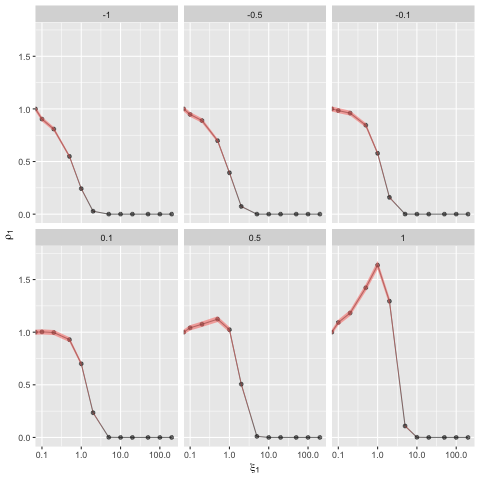
\includegraphics[width = 0.7\textwidth]{fig/rho_1_beta.png}
\label{fig:rho_1_beta}
\end{figure}

\begin{figure}[H]
\centering
\caption{Representation of $\tilde\densityratio_{\lbrace 1\rbrace}(\position\mid\signal)$ when $\Sample \sim \mathrm{bpp}(\Desvar,\samplesize)$, $\paramnuisance_{1} = 1$, and $\paramnuisance_{2}$ varies. The value of $\signal$ is reported on top of the corresponding graph.}
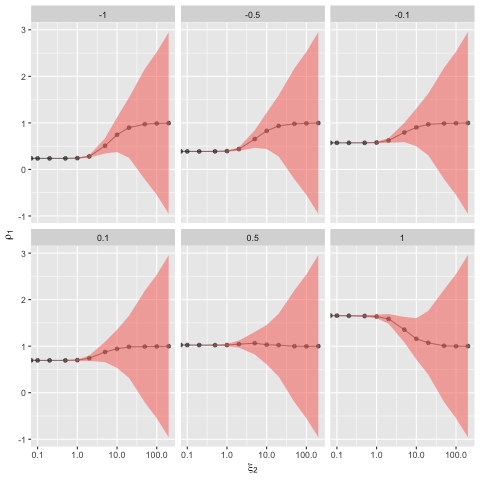
\includegraphics[width = 0.7\textwidth]{fig/rho_1_gamma.png}
\label{fig:rho_1_gamma}
\end{figure}

%\begin{example}{(continued)}
%We remark that $\paramnuisance_1=0$ implies the independence of $\Desvar$ and $\Signal$. 
%By continuity
%\begin{figure}[H]
%\caption{Estimation of $\densityratio_{\{1\}}(\signal\mid\position;\parampop,\paramnuisance)$}
%\end{figure}
%\end{example}

\begin{figure}[H]
\centering
\caption{Representation of $\tilde\densityratio_{\lbrace 1,2\rbrace}(\position\mid\signal)$ when $\Sample \sim \mathrm{bpp}(\Desvar,\samplesize)$, $\paramnuisance_{1} = 1$, $\paramnuisance_{2}=1$, and for four different couples of points.}
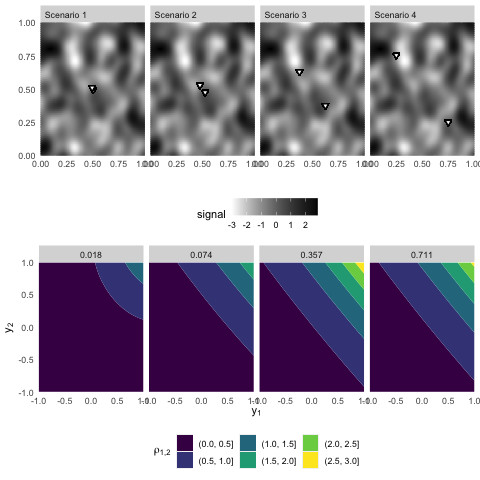
\includegraphics[width = 0.8\textwidth]{fig/rho_12_contour.png}
\label{fig:rho_12}
\end{figure}







%\subsection{Distribution of $\Signal[\Sample]$}
\subsection{Density ratio $\densityratio$ and distribution of \texorpdfstring{$\Signal[\Sample]$}{Y[\Sample_\Sampleindex]} }
The density of $\Signal[\Sample_\Sampleindex]$ with respect to $\dominantYbar$ is defined by
\begin{eqnarray}\density_{\Sample_\Sampleindex,\Signal[\Sample_\Sampleindex]}(\position\mid\signal)&=& \density_{\Signal[\position]}(\signal)~\times~\densityratio_{\Sampleindex}(\position\mid\signal)~\times~\density_{\Sample_\Sampleindex}(\position).\label{eq:iuhsdewripeowi}\\
&=& \density_{\Signal[\position]}(\signal)~\times~\density_{\Sample_\Sampleindex\mid\Signal[\position]}(\position\mid\signal).\label{eq:iuhsdewripeowi2}
\end{eqnarray}

In particular,
\begin{eqnarray}\density_{\Sample,\Signal[\Sample]}(\position\mid\signal)&=& \density_{\Signal[\position]}(\signal)~\times~\densityratio_{\{1,\ldots,\Samplesize\}}(\position\mid\signal)~\times~\density_{\Sample}(\position)
.\label{eq:iuhsdewripeowi3}
\end{eqnarray}


So when $\Desvar\perp\Signal$,
\begin{equation}\density_{\Signal[\Sample_\Sampleindex]\mid\Sample_\Sampleindex}(\signal\mid \position)= \density_{\Signal[\position]}(\signal).\label{eq:iuhsdewripeowi2}\end{equation}

\cite{pfefferman_1992} explore  the case where
$K=\{1\}$ and the spatial process satisfies the  population independence assumption:

$\forall \position\in\Pop^{\{1,\ldots,\samplesize\}}$, such that $(\position[1],\ldots,\position[\samplesize])$ are two by two  distinct,

\begin{equation}
(\Signal[\position[1]],\ldots,\Signal[\position[\samplesize]])\text{ are i.i.d variables}.
\label{eq:independenceassumption}
\end{equation}

To the ``population'' distribution, which is the distribution of $\Signal$ that satisfies Equation \eqref{eq:independenceassumption} with probability density function $\density_{\Signal[\position]}$ for $\position \in\Pop^{\{1\}}$, \cite{pfefferman_1992} oppose the sample distribution, that is the  distribution of a random variable $\Signal^\star$ that satisfies Equation \eqref{eq:independenceassumption}  and with probability density function  $\densityratio_{\{1\}}\density_{\Signal[\position]}$ for $\position \in\Pop^{\{1\}}$.

The random variable $\Signal^\star$ ''does not exist``, in the sense that if the observer could measure $\Signal[\position]$ for all values of $\position$ on $\Pop$, of for values of $\position$ in a non informative sample (e.g. such that $\densityratio=1$), the distribution of  observations would have probability density $\density_\Signal[\Sample]$.
With an informative sample, the observations are similar to what one would observe with a simple random sample and if the population was following $P^{\Signal^\star}$ and not $P^\Signal$. The distribution of $\Signal^\star$ is called by \cite{pfefferman_1992} the ``sample'' distribution.

In the case of a spatial process, can we define a sample distribution ?

Sometimes not, due to the property pointed out in Remark \ref{remark:K1subsetK2}:
the finite dimensional probability density functions 
$\densityratio{\{1,\ldots,\samplesize\}}(\position\mid\signal)\density_{\Signal[\position](\signal)}$ are not necessarily the finite dimensional densities of the same random process distribution.
A sufficient condition for the finite dimensional densities to be finite dimensional probability functions of the same process is that the sample size is fixed.
But then, there is not necessarily unicity of the random process distribution that have these finite dimensional probability density functions, as they are only defined up to the dimension equal to the sample size.



Generalising \cite{pfefferman_1992}, the selection is non informative when $\forall \uple\in\mathbb{N}$ $P^{\Signal[\Sample],\Sample}-\text{a.s.}(\signal,\position)$, $$\densityratio_{\{1,\ldots,\Samplesize\}}(\position\mid\signal)=1.$$ In this case, we consider that the sample distribution corresponds to the population distribution.


In the general case, we then define the sample distribution as a
collection of finite dimensional distributions with respective p.d.f.'s
$\densityratio{\{1,\ldots,\samplesize'\}}(\position\mid\signal)\density_{\Signal[\position](\signal)}$, with\\ $\samplesize'\in\left\{\{1,\ldots,\max\left(\Samplesize(\Samplesize^{-1}(\mathbb{N}))\right)\right\}$. 



%\subsection{Sample Variogram}
\subsection{Sample counterpart of distribution characteristics}

Even if the definition of the sample distribution is not the distribution of a random process on $\Pop$, we propose to define the sample counterpart of different characteristics of the population distribution as for example %the intensity and 
the sample semivariogram.


In a non spatial framework,  \cite{pfefferman_1992} differentiates the characteristics of the distribution of one variable when observed on the sample, and the characteristics of the same variable when observed on the population. The terminology to differentiate consists in adding ``populatio'' or ``sample'' to the name of the characteristic. For example, the population probability density function (pdf) is the equivalent  $\density_{\Signal[\position]}$ in our example, and the sample pdf is the density $\density_{\Signal[\Sample[1]]}$. \cite{bonnery2012uniform} and \cite{dbb1} investigate further this concept of population and sample characteristics.
In the following, we provide the definition of the sample characteristics of the distribution of $\Signal$ that are meaningful in the context of a spatial model.



%\subsubsection{Sample probability density function, and cumulative density function}
Some characteristics of the distribution of $\Signal$ can be  defined as expected values of a transformation of the values of $\Signal$ on all samples of $\Pop$.
For example, we have seen that the distribution of 
a Gaussian process is characterised by $E[\Signal[\position]]$ for $\position\in \Pop$ and
$\Var[\Signal[\position]]$ for $\position\in \Pop^{\{1,2\}}$. Those characteristics can be obtained by integrals of the form $\int g(\signal[\position]) \density_{\Signal[\position]}(\signal[\position])\derive\dominantYbar$, which themselves can be seen as expected values of statistics derived from the values of $\Signal$ on a simple random sample with replacement.
Those characteristics are called ``population characteristics''. Their sample counterparts are obtained by substituting $ \density_{\Signal[\position]}$ by $\densityratio_{\{1,\ldots,\size(\position)\}}\density_{\Signal[\position]}$, and can be interpreted as the expected value of the same statistics derived from the values of $\Signal$ on the informative sample $\Sample$.





%In the i.i.d. case, where the realisation for each units of the population is i.i.d.
%Generalising \cite{bonnery2012uniform}, we can define the averaged sample probability distribution (p.d.f) as 
%$\signal\mapsto\sum_{\samplesize\geq 1}P(\Samplesize=\samplesize)(\derive P^{\Signal[\Sample[1]]\mid \Samplesize=\samplesize}/\derive\dominantY)(\signal)$
%by opposition to the population averaged pdf 
%$\signal\mapsto\int (\derive P^{\Signal[\position]/}\derive\dominantY)(\signal)\derive \dominantU(\position)$, 
%as well as the sample probability density function of $\Signal[\position]$ as
%$\signal\mapsto(\derive P^{\Signal[S[1]]\mid\Samplesize[1]=\position}/\derive\dominantY)(\signal)$
%by opposition to the ``population`` pdf of $\Signal[\position]$ 
%$\signal\mapsto(\derive P^{\Signal[\position]}/\derive\dominantY)(\signal)$


%We define the cumulative distribution function of the sample distribution is 
%the function $\alpha\mapsto\sum_{\samplesize\geq 1}P(\Samplesize=\samplesize)\times  P(\Signal[\Sample[1]]\leq\alpha\mid \Samplesize=\samplesize)$.

%\begin{property}
%The sample probability density function is $\densityratio_{\{1\}}(\position\mid\signal)\density_{}$
%\end{property}

%\subsubsection{Sample Intensity}

%\subsubsection{Semivariogram of the sample distribution}
In the case of sampling with fixed size $\samplesize\geq 2$, 
define the sample semivariogram for exchangeable designs as 
$$\Semivariogram^\star(h)=\frac12~\E\left[\left(\Signal[\Sample[1]]-\Signal[\Sample[2]]\right)^2\mid \Sample[2]-\Sample[1]=h \right].$$

In the case of a random size sample, one can define the sample semivariogram as 
$$\Semivariogram^\star(h)=\frac12\sum_{\samplesize\geq2}P(\Samplesize=\samplesize)~\E\left[\left(\Signal[\Sample[1]]-\Signal[\Sample[2]]\right)^2\mid \Samplesize=\samplesize \text { and }\Sample[2]-\Sample[1]=h \right].$$

\begin{property}[Relationship between $\Semivariogram$, $\Semivariogram^\star$ and $\densityratio$]
$$\Semivariogram^\star(h)=\frac12\int_{\Pop^{\{1,2\}}} \left[\int_{\range{\Signal}^{\{1,2\}}} (\signal(2)-\signal(1))^2~ \density_{\Signal[\position]}(\signal)~
\intensityratio_{\{1,2\}}(\position\mid\signal)~
\derive\dominantY^{\otimes 2}(\signal)
\right] \derive(\dominantU^{\otimes\{1, 2\}})^{X\mid X[2]-X[1]=h}(\position)$$
\end{property}

\begin{proof}
Let $\position\in\Pop^{\{1,2\}}$, then
\begin{eqnarray*}
\lefteqn{\E\left[\left(\Signal[\position(2)]-\Signal[\position(1)]\right)^2\mid \Sample_{\{1,2\}}=\position\right]}\\
&=&\int_{\range{\Signal}^2} (\signal(2)-\signal(1))^2~
\density_{\Signal[\position]\mid S_{\{1,2\}}}(\signal\mid \position)~
\derive\dominantY^{\otimes\{1, 2\}}(\signal) \\
&=&\int_{\range{\Signal}^2} (\signal(2)-\signal(1))^2~
\densityratio_{\{1,2\}}(\position\mid\signal)~ \density_{\Signal[\position]}(\signal)~
\derive\dominantY^{\otimes\{1, 2\}}(\signal) \\
\end{eqnarray*}
\end{proof}

%\subsubsection*{Example (continued)}
%
%Define the approximated sample variogram by replacing $\densityratio_{\{1,2\}}$ by $\tilde{\densityratio_{\{1,2\}}}$ in the expression of the sample variogram:
%$$\tilde\Semivariogram(h)^\star=
%\Semivariogram(h)
%\int\left(\int
%(\signal'(2)-\signal'(1))^2~ \frac{\mathrm{e}^{-\frac{(\signal')_1^2+(\signal')_2^2}{2}}}{2\pi}~
%\derive\dominantY^{\otimes \{1,2\}}(\signal')\right). 
%$$
%
%\begin{proof}
%See Appendix \ref{labelnotdoneyet}
%\end{proof}





%\subsubsection{Integrated mean if the sample distribution}

%The  integration of the population process is defined as
%$$\int_\Pop \Signal(\position)\derive\dominantU(\position).$$
%The prediction of $\int_\Pop \Signal(\position)\derive\dominantU(\position)$ is an important matter in survey sampling, it is the prediction of the sum of a characteristic of the population over the population. 

%In the case of unicity of the distribution of $\Signal^\star$, the integration of the sample process is defined as a random variable of the form
%$\int_\Pop \Signal^\star(\position)\derive\dominantU(\position)$.
%where $\Signal^\star$ satisfies Equation \eqref{def:sampleprocess}.

